\documentclass[math]{answer}

\begin{document}

\helloworld{104}{臺北市立建國高級中學}{科學班}{數學}

\section{多重選擇題}

\begin{questions}
	\question
	\answer{(2)(4)(5)}{3}{
		因為$a + b = 800$,我們可以把題目的$b$用$800 - a$換掉,得到
		\[
			a, 800 - a, c, 800 - c, 800 + c - 2a, 2a + c - 800, 800 + c
		\]
		為兩兩不同的質數。

		\begin{choices}
			\choice $c = 3$時,這七個質數變為
			\[
				a, 800 - a, 3, 797, 803 - 2a, 2a - 797, 803.
			\]
			注意到質數最小為$2$,因此$803 - 2a, 2a - 797 \geq 2$。滿足條件的整數只有$400$,所以$a = 400$,不是質數。這代表$c = 3$是不可能成立的。
			\choice 注意到如果$c$除以$3$的餘數不是$2$,則只會有以下兩個可能:
			\begin{itemize}
				\item $c$除以$3$的餘數是$1$:那$800 + c$就是一個$3$的倍數。但是,$800 + c$是一個比$800$還大的質數,所以不可能是$3$的倍數。
				\item $c$是$3$的倍數:那只有$c = 3$這種可能(因為$c$是質數)。由選項(1)可以知道這是不可能的。
			\end{itemize}
			因此,此選項正確。
			\choice 我們進一步觀察選項(2)的結果,可得到$800 - c$必為$3$的倍數,而唯一符合條件的質數只有$3$,所以$800 - c = 3$,得$c = 797$。所以
			\[
				a, 800 - a, 797, 3, 1597 - 2a, 2a - 3, 1597
			\]
			皆為質數。如果這七個質數有一個是$2$,那只可能是$a$或$800 - a$(因為從上面的表示法,可以看出其他五個都是奇數)。無論是哪個,都會造成另一個不是質數的情形,因此不可能發生。
			\choice 這選項其實挺無聊的(當然,你要先求出$c$才會覺得它無聊啦)。當$a = 13, b = 787$時,以上七個質數變為$13, 787, 797, 3, 1571, 23, 1597$,都是兩兩相異的質數。
			\choice 從選項(3),我們可以得到$a$的範圍為$3 \leq a < 797$ (因為以上每一個質數皆大於$2$)。所以最大的數字為$1597$、最小為$3$,即$d$最大可能為$1594$。
		\end{choices}
	}

	\question
	\answer{(1)(2)(5)}{2.5}{
		首先,可以發現四邊形$ED^\prime MF$和四邊形$EDCF$全等。再來,我們令$\overline{MC}$和$\overline{EF}$交於$P$點。
		\begin{choices}
			\choice 可以發現$\overline{CM} \perp \overline{EF}$(因為$C$對折後就變$M$)。因此,$\frac{\overline{MC} \times \overline{EF}}{2}$就是四邊形$EMFC$的面積。再來,可以發現$\triangle EFC$的面積即為$\frac{\overline{AB} \times \overline{FC}}{2}$,因此四邊形$EMFC$的面積(也等於兩倍$\triangle EFC$的面積)即為$\overline{AB} \times \overline{FC} = \overline{AB} \times \overline{MF}$。結合兩式,即得到$\overline{MC} \times \overline{EF} = 2\overline{MF} \times \overline{AB}$。
			\choice 因為$\overline{CM} \perp \overline{EF}$,所以$\angle MPF = \ang{90}$。於是$\angle MPF + \angle MBF = \ang{180}$,即$M, P, B, F$四點共圓。由圓外冪關係可得(注意$\overline{MP} = \overline{PC} = \frac{1}{2}\overline{CM}$)
			\[
				\overline{BC} \times \overline{FC} = \overline{CP} \times \overline{CM} = \frac{\overline{MC}^2}{2}.
			\]
			整理後,即可以發現此選項正確。
			\choice 令$\overline{MF} = \overline{CF} = x, \overline{AM} = \overline{MB} = y$,則由前兩個選項可得
			\[
				\begin{cases}
					\overline{MC} \times 6 = 2 \cdot \overline{MF} \times \overline{AB} = 4xy \\
					\overline{MC}^2 = 16 \times \overline{FC} = 16x
				\end{cases}
			\]
			將兩式相除後整理得$24 = \overline{MC} \times y = \sqrt{64 + y^2} \times y$,因此$y = 2\sqrt{2}$。於是
			\[
				\overline{ED} = \overline{FC} - \sqrt{\overline{EF}^2 - \overline{AB}^2} = \frac{5}{2},
			\]
			這代表$\overline{AE} : \overline{ED} = \frac{11}{2} : \frac{5}{2} \neq 5 : 3$。
			\choice 可以發現$\triangle D^\prime EN, \triangle AMN, \triangle BFM$都互為相似三角形,因此我們只要判斷$\overline{D^\prime E} : \overline{AM} : \overline{BF}$是否為$5 : 6 : 7$即可。然而,由先前的結果,我們可以發現$\overline{D^\prime E} : \overline{AM} : \overline{BF} = \frac{5}{2} : 2\sqrt{2} : \frac{7}{2}$,故此選項不正確。
			\choice 我們先算出$\triangle D^\prime EN$的面積。由第四個選項,我們可以知道$\triangle D^\prime EN$和$\triangle MBF$的面積比為$25 : 49$。又$\triangle MBF$的面積為
			\[
				\frac{2\sqrt{2} \times \frac{7}{2}}{2} = \frac{7\sqrt{2}}{2},
			\]
			故$\triangle D^\prime EN$面積為$\frac{25\sqrt{2}}{14}$。

			因此,所求即為梯形$DEFC$的面積扣除$\frac{25\sqrt{2}}{14}$:
			\[
				\frac{\left(\frac{5}{2} + \frac{9}{2}\right) \times 4\sqrt{2}}{2} - \frac{25\sqrt{2}}{14} = \frac{171}{14}\sqrt{2}.
			\]
		\end{choices}
	}
\end{questions}

\section{填充題}

\begin{questions}
	\question
	\answer{18}{1.5}{
		可以發現第$n$個橫列的數字會形成首項為$2n - 1$、公差為$n + 1$的等差數列。於是,根據等差數列的公式,第$n$橫列的第$m$項為
		\[
			(2n - 1) + (m - 1)(n + 1) = mn + m + n - 2 = (m + 1)(n + 1) - 3.
		\]
		所以,我們要找出有多少組不同的正整數數對$(m, n)$會讓$(m + 1)(n + 1) - 3 = 1533$,即$(m + 1), (n + 1)$為$1536$的因數。因為$1536 = 2^9 \cdot 3$有$(9 + 1)(1 + 1) = 20$個因數,所以總共有$20 - 2 = 18$種可能。(最後扣除$2$的原因是$1$和$1536$兩個因數會使$m$或$n$變為$0$)。
	}

	\question
	\answer{$-18, -3, -\frac{23}{8}$}{2}{
		我們先觀察方程式
		\begin{equation}
			\label{eq:2-2-1}
			\frac{x + 2}{x - 2} + \frac{x - 1}{x + 1} + \frac{3x + a}{x^2 - x - 2} = 0.
		\end{equation}
		因為分母不可為$0$,故$x \neq 2, -1$。將$\eqref{eq:2-2-1}$兩邊同乘$x^2 - x - 2$後整理,得到
		\begin{equation}
			\label{eq:2-2-2}
			(x + 2)(x + 1) + (x - 2)(x - 1) + (3x + a) = 0; \quad 2x^2 + 3x + (4 + a) = 0.
		\end{equation}
		題目說只有一個$x$滿足$\eqref{eq:2-2-1}$,故$\eqref{eq:2-2-2}$的判別式要嘛為$0$:
		\begin{equation}
			\label{eq:2-2-3}
			9 - 8(4 + a) = 0; \quad a = -\frac{23}{8}
		\end{equation}
		要嘛判別式大於$0$,但是有其中一解為$2, -1$(記得這兩個數字會讓原式分母為$0$,故不為原方程式解)。這代表將$x$代入$2, -1$時,$\eqref{eq:2-2-3}$為$0$:
		\begin{equation}
			\label{eq:2-2-4}
			18 + a = 0, 3 + a = 0.
		\end{equation}
		綜合$\eqref{eq:2-2-3}$和$\eqref{eq:2-2-4}$,得到$a = -18, -3, -\frac{23}{8}$,代回皆成立。
	}

	\question
	\answer{1679}{3}{
		我們先觀察到一個事實:當$a$為定值時,$|k|$愈大代表$(a + k)^2 + (a - k)^2$愈大。舉例來說,$6^2 + 5^2 < 7^2 + 4^2 < 8^2 + 3^2$。

		現在,我們有$x_1 + x_2 + \dots + x_{31} = 197$這個條件。我們的目標是找到$M = x_1^2 + \dots + x_{31}^2$的最大值。假設說這31個數中,我們找的到兩個不是$1$也不是$9$的數$x_i$和$x_j$(假設$x_i \geq x_j$),那我們可以發現
		\[
			x_i^2 + x_j^2 < \left(x_i + 1\right)^2 + \left(x_j - 1\right)^2 < \dots.
		\]
		這代表說當我們將$x_i$和$x_j$的距離「擴大」(變成$x_i + k$和$x_j - k$,$k$為正整數)時,可以讓$M$的值變大,且擴大後的$31$個數總和仍為$197$。於是,我們可以對以上$31$個數做以下操作:
		\begin{enumerate}
			\item 若在這$31$個數中,我們找的到兩個不是$1$或$9$的數,那我們就將這兩個數「擴大」,直到這兩個數有其中一個變成$1$或$9$。擴大後的$31$個數總和仍然是$197$,但是平方和變大了。
			\item 重複以上步驟,直到只剩下$1$個或$0$個數不是$1$或$9$。
		\end{enumerate}
		假設最後的$31$個數中,有$a$個$1$、$b$個$9$和一個不知道是多少的數(假設這個數是$c$;$c$也有可能為$1$或$9$)。於是,
		\[
			\begin{cases}
				a + 9b + c & = 197 \\
				a + b      & = 30.
			\end{cases}
		\]
		兩式相減後得$8b + c = 167 = 8 \times 20 + 7$。又因為$1 \leq c \leq 9$且$b, c$都是正整數,所以$c = 7$。代回後得$b = 20, a = 10$,故$M$的最大值為$20 \times 9^2 + 10 \times 1^2 + 7^2 = 1679$。
	}

	\question
	\xanswer{48}{2.5}{
		題目要我們找出$\left[\frac{2015}{n}\right]$湊不出來的最小整數。當$n$愈大時,$\left[\frac{2015}{n}\right]$會愈來愈密集,最後變為$0$。我們當然可以用試的來找出$k$的最小值(如果你數感夠好,還可以感覺到$k$大概在$\sqrt{2015}$附近。詳見補充),但是以下提供一個方法來判斷$k$的最小值大概在哪裡。

		首先,我們觀察$\left\lfloor\frac{2015}{n}\right\rfloor = k$這個式子。我們可以將它化為
		\[
			k \leq \frac{2015}{n} < k + 1; \quad \frac{2015}{k + 1} < n \leq \frac{2015}{k}.
		\]
		如果$\frac{2015}{k} - \frac{2015}{k + 1} \geq 1$的話,我們一定可以在$\frac{2015}{k}$和$\frac{2015}{k + 1}$中間發現一個整數(聽起來很合理吧,兩個連續整數的差就只有1而已)。如此一來,這個整數就是原方程式的一個整數根,矛盾。於是,我們有$\frac{2015}{k} - \frac{2015}{k + 1} < 1$:
		\begin{equation}
			\label{eq:2-4-2}
			2015 < k(k + 1); \quad k \geq 45. \quad \text{(因為$k$為整數)}
		\end{equation}

		再來,我們就可以從$45$一個一個試了。
		\begin{table}[H]
			\centering
			\begin{tabular}{ccccc}
				\toprule
				$k$                  & 45 & 46 & 47 & 48 \\
				\midrule
				$\frac{2015}{k}$     & 44 & 43 & 42 & 41 \\
				$\frac{2015}{k + 1}$ & 43 & 42 & 41 & 41 \\
				\bottomrule
			\end{tabular}
		\end{table}
		可以發現當$k = 48$時,沒有正整數$n$滿足$\frac{2015}{k + 1} < n \leq \frac{2015}{k}$,故所求即為$48$。
	}{
		\begin{itemize}
			\item 只要看到高斯符號的題目,都應該要先想到$[k] \leq k < [k] + 1$這個式子。它可以幫助你把高斯符號轉為正常的不等式。
			\item 關於數感的部分(以下的說明都不是非常嚴謹,只是一些我做這題時的想法,大家可以參考一下,看不懂也不是你的錯):誠如詳解所述,$\left\lfloor \frac{2015}{n} \right\rfloor$會隨著$n$變大而減緩改變的幅度。我們要找到的是數列$\left\lfloor \frac{2015}{1} \right\rfloor, \left\lfloor \frac{2015}{2} \right\rfloor,\dots$中,沒有出現的正整數中最小的那一個。這時的$n$應該要讓$\left\lfloor \frac{2015}{n} \right\rfloor$和$\left\lfloor \frac{2015}{n+1} \right\rfloor$恰好跳過一個正整數。於是$\left\lfloor \frac{2015}{n} \right\rfloor - \left\lfloor \frac{2015}{n + 1} \right\rfloor\approx 1.\dots$。所以,這時的$n, k$應該都要是在$\sqrt{2015}$附近。如果不懂的話,那就代幾個數字進去看看吧,我盡力了。
		\end{itemize}
	}

	\question
	\answer{$115, 625$}{2.25}{
		從題目的條件,我們可以得到$n$是$5$的倍數。所以$c = 0, 5$。

		\begin{parts}
			\part
			當$c = 0$時:可以得到
			\begin{equation}
				\label{eq:2-5-1}
				n = 100a + 10b = 5f(n) = 5(a + b + ab); \quad 19a = b(a - 1).
			\end{equation}
			由於$b$和$a - 1$皆不可能為$19$的倍數,我們可以發現此情況不可能發生。
			\part
			當$c = 5$時:可以得到
			\begin{equation}
				\label{eq:2-5-2}
				n = 100a + 10b + 5 = 5f(n) = 5(a + b + 5 + ab + 5a + 5b + 5ab); \quad 7a = 2b + 2 + 3ab.
			\end{equation}
			由$\eqref{eq:2-5-2}$,我們可以發現$7a > 3ab$,故$b = 1, 2$。當$b = 1$時,得到$7a = 4 + 3a$,即$a = 1$、$n = 115$。當$b = 2$時,得到$7a = 6 + 6a$,即$a = 6$、$n = 625$。
		\end{parts}
		綜上,$n = 115, 625$,代回皆成立。
	}

	\question
	\answer{
		$\left(\frac{1048575}{1048576}, 1, \frac{1}{4}\right)$
	}{3.5}{
		我們先將原式整理一下,得到
		\begin{equation}
			\label{eq:2-6-1}
			(2x + 1)^{20}=(ax + b)^{20} + (x^2 + px + q)^{10}.
		\end{equation}
		再來,我們將$x$代入$-\frac{1}{2}$以把左式消掉,得
		\[
			0 = \left(\frac{-1}{2}a + b\right)^{20} + \left(\frac{1}{4} + \frac{-1}{2}p + q\right)^{10}.
		\]
		因為右式是兩個平方式的相加,所以只有在它們都為$0$時,上式才可能成立。於是,
		\begin{equation}
			\label{eq:2-6-2}
			b = \frac{1}{2}a, \quad \frac{1}{4} + \frac{-1}{2}p + q = 0.
		\end{equation}

		再來,觀察$\eqref{eq:2-6-1}$的首項($x^{20}$)係數,可以得到$2^{20} = a^{20} + 1$,故
		\[
			b^{20} = \frac{a^{20}}{2^{20}} = \frac{2^{20} - 1}{2^{20}} = \frac{1048575}{1048576}.
		\]
		此外,我們有(注意$b = \frac{1}{2}a$)
		\[
			(ax + b)^{20} = \frac{a^{20}}{2^{20}} \left(2x + 1\right)^{20} = \frac{2^{20} - 1}{2^{20}}(2x + 1)^{20},
		\]
		代回$\eqref{eq:2-6-1}$後,得到
		\[
			(x^2 + px + q)^{10} = \frac{1}{2^{20}}(2x + 1)^{20} = \left(x + \frac{1}{2}\right)^{20} = \left(x^2 + x + \frac{1}{4}\right)^{10},
		\]
		故$p = 1, q = \frac{1}{4}$。
	}
\end{questions}

\section{計算證明題}

\begin{questions}
	\question
	\sprout{
		(1) $\frac{81}{4}, P\left(\frac{9}{2}, \frac{7\sqrt{3}}{2}\right)$
		\nextitem
		(2) $2$
	}
	在開始第一小題前,相信大家都可以得到$\angle BAO = \ang{60}$(因為$\triangle BOA$是正三角形)。於是$\angle CAO = \angle CAB + \angle BAO = \ang{90}$,即$\overline{CA} \perp \overline{OA}$。又因為$\triangle CBA$是$\ang{30}$-$\ang{60}$-$\ang{90}$的直角三角形,故$\overline{CA} = \frac{2}{\sqrt{3}}\overline{BA} = \frac{16}{\sqrt{3}}$。因此,$C\left(8, \frac{16}{\sqrt{3}}\right)$。
	\begin{parts}
		\part
		\eanswernl{1.5}{
			當$P$還在$\overline{AB}$上時,我們令$\overline{AP} = \overline{DQ} = k$。可以得到$P\left(8 - \frac{k}{2}, \frac{\sqrt{3}}{2}k\right)$。則$\triangle OPQ$的面積為$P$點$x$座標乘上$\overline{OQ}$再除以2。於是,$\triangle OPQ$面積為
			\[
				\frac{\left(8 - \frac{k}{2}\right)(2 + k)}{2} = -\left(\frac{k}{2} - \frac{7}{2}\right)^2 + \frac{81}{4},
			\]
			最大值為$\frac{81}{4}$,發生在$k = 7$時。此時$P\left(\frac{9}{2}, \frac{7\sqrt{3}}{2}\right)$。
		}
		\part
		\eanswernl{3}{
			\begin{itemize}
				\item 當$P$在$\overline{AB}$上時:

				      由題目說明,我們可以發現此時$\angle OPQ$的大小會隨著$t$的增大而增大。又$P$在$A$點上時,$\angle OPQ < \ang{90}$,而$P$在$B$點上時,$\angle OPQ > \ang{90}$,所以洽有一個點滿足$\angle OPQ = \ang{90}$。
				\item 當$P$在$\overline{BC}$上時:

				      當$Q(0, 2 + k)$時,我們可以得到
				      \[
					      P\left(4 + \frac{\sqrt{3}}{2}(k - 8),4\sqrt{3} + \frac{1}{2}(k - 8)\right) = \left(4 - 4\sqrt{3} + \frac{\sqrt{3}}{2}k, 4\sqrt{3} - 4 + \frac{k}{2}\right).
				      \]
				      要使$\angle OPQ = \ang{90}$,$\triangle OPQ$要為一個直角三角形,故其外心在$O, Q$中點,外接圓半徑為$\frac{\overline{OQ}}{2} = \frac{k + 2}{2}$。於是,$P$和$O, Q$中點的距離要為$\frac{k + 2}{2}$:
				      \[
					      \left(4 - 4\sqrt{3} + \frac{\sqrt{3}}{2}k\right)^2 + \left(4\sqrt{3} - 4 + \frac{k}{2} - \frac{k}{2}\right)^2 = \left(\frac{k + 2}{2}\right)^2.
				      \]
				      共有一個點滿足以上方程式。
			\end{itemize}
			綜上,共有兩個點滿足題意。
		}
	\end{parts}

	\question
	\answer{$864, 2736$}{3}{
		首先,可以發現滿意度為$1, 2, 5, 6, 7$的排法是不存在的(滿意度為$1, 2$時,第三個人一定還可以順心的選座位,而四個人順心的選坐坐位後,第五個人一定沒辦法順心的選坐位)。因此,我們只要解決滿意度為$3$和$4$的作法即可。
		\begin{itemize}
			\item 滿意度為$4$的座位排法:

			      坐完四個人之後,座位的分布一定是如下:
			      \begin{table}[H]
				      \centering
				      \begin{tabular}{|p{0.3cm}|p{0.3cm}|p{0.3cm}|p{0.3cm}|p{0.3cm}|p{0.3cm}|p{0.3cm}|}
					      \hline
					      $\odot$ & ~ & $\odot$ & ~ & $\odot$ & ~ & $\odot$ \\
					      \hline
				      \end{tabular}
			      \end{table}
			      其中$\odot$是有人坐的座位。因此,$1, 2, 3, 4$要放在這四個位子(共有$4! = 24$種放法),而$5, 6, 7$要放在剩下的三個位子(共有$3! = 6$種放法),共有$24 \times 6 = 144$種方法。
			\item 滿意度為$3$的座位排法:

			      坐完三個人後,座位的分布有以下五種:
			      \begin{table}[H]
				      \centering
				      \begin{tabular}{|p{0.3cm}|p{0.3cm}|p{0.3cm}|p{0.3cm}|p{0.3cm}|p{0.3cm}|p{0.3cm}|}
					      \hline
					      $\odot$ & ~ & $\odot$ & ~ & ~ & $\odot$ & ~ \\
					      \hline
				      \end{tabular}
				      \begin{tabular}{|p{0.3cm}|p{0.3cm}|p{0.3cm}|p{0.3cm}|p{0.3cm}|p{0.3cm}|p{0.3cm}|}
					      \hline
					      ~ & $\odot$ & ~ & ~ & $\odot$ & ~ & $\odot$ \\
					      \hline
				      \end{tabular}
			      \end{table}
			      \begin{table}[H]
				      \centering
				      \begin{tabular}{|p{0.3cm}|p{0.3cm}|p{0.3cm}|p{0.3cm}|p{0.3cm}|p{0.3cm}|p{0.3cm}|}
					      \hline
					      $\odot$ & ~ & ~ & $\odot$ & ~ & $\odot$ & ~ \\
					      \hline
				      \end{tabular}
				      \begin{tabular}{|p{0.3cm}|p{0.3cm}|p{0.3cm}|p{0.3cm}|p{0.3cm}|p{0.3cm}|p{0.3cm}|}
					      \hline
					      ~ & $\odot$ & ~ & $\odot$ & ~ & ~ & $\odot$ \\
					      \hline
				      \end{tabular}
			      \end{table}
			      \begin{table}[H]
				      \centering
				      \begin{tabular}{|p{0.3cm}|p{0.3cm}|p{0.3cm}|p{0.3cm}|p{0.3cm}|p{0.3cm}|p{0.3cm}|}
					      \hline
					      $\odot$ & ~ & ~ & $\odot$ & ~ & ~ & $\odot$ \\
					      \hline
				      \end{tabular}
			      \end{table}
			      依照先前的算法,共有$5 \times (3! \times 4!) = 720$種方法。
		\end{itemize}
		綜上,共有$144 + 720 = 864$種滿意次序坐法,且滿意度總和為$144 \times 4+720 \times 3 = 2736$。
	}

	\question
	\sprout{見詳解}
	\begin{parts}
		\part
		\panswernl{2.5}{
			\begin{itemize}
				\item 因為$O_3$是$\triangle ABI$的外接圓圓心,所以$2\angle AIB + \angle AO_3B = \ang{360}$(提示:考慮這兩個角對到$\triangle ABI$外接圓的圓弧,$\angle AIB = \frac{1}{2}\arc{AB}$(和$I$不同邊的那一個$\arc{AB}$)、$\angle AO_3B = \arc{AIB}$,而這兩個弧合起來剛好是一整個圓)
				\item 因為$I$為$\triangle ABC$的內心,所以$\angle AIB = \ang{90} + \frac{1}{2}\angle ACB$(還是提示:$I$是角平分線的交點,所以$\angle AIB = \ang{180} - \angle BAI - \angle IBA = \ang{180} - \frac{1}{2}\angle BAC - \frac{1}{2}\angle CBA$)。
			\end{itemize}
			將兩個條件結合後,可得$\angle AO_3B + \angle ACB = \ang{180}$,故$A, B, C, O_3$四點共圓。同理,可得到$A, B, C, O_2$、$A, B, C, O_1$四點共圓,因此$A, B, C, O_1, O_2, O_3$六點共圓。於是,$\triangle ABC$和$\triangle O_1O_2O_3$有相同的外接圓,當然也有相同的外接圓圓心。
		}
		\part
		\exanswernl{3.75}{
			如果$A, B, H, I$要四點共圓,那$\angle AHB = \angle AIB$或是$\angle AHB + \angle AIB = \ang{180}$。從前一小題,我們得到$\angle AIB = \ang{90} + \frac{1}{2}\angle ACB$,而我相信你們都能發現$\angle AHB = \ang{180} - \angle ACB$(看不出來的話,就把三條高都畫出來吧)。於是,我們可以得到$\angle ACB = \ang{60},\ang{180}$。顯然只有$\ang{60}$符合條件。

			那要如何畫出讓$\angle ACB = \ang{60}$的軌跡呢?相信大家都想的到當$\triangle ABC$為正三角形時,$\angle C = \ang{60}$,因此我們先畫出:
			\begin{figure}[H]
				\centering
				\begin{tikzpicture}[scale=0.5]
					\draw[line width=0.5pt] (0, 0) -- (3, 0);
					\node at (0, 0)[anchor = north east] {$A$};
					\node at (3, 0)[anchor = north west] {$B$};
					\draw[color = gray, line width=0.5pt, dashed] (0, 0) -- (1.5, 2.6) -- (3, 0) -- (1.5, -2.6) -- (0, 0);
					\filldraw[black] (1.5,2.6) circle (1pt);
					\filldraw[black] (1.5,-2.6) circle (1pt);
				\end{tikzpicture}
			\end{figure}
			再來,如果把這兩個正三角形的外接圓畫出來的話,你會發現$C$點的軌跡一定在這兩個圓上(不然$\angle ACB \neq \ang{60}$)。所以$C$的軌跡即為
			\begin{figure}[H]
				\centering
				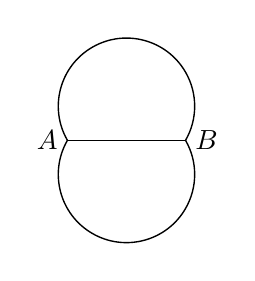
\begin{tikzpicture}[scale=0.5]
					\draw[line width=0.5pt] (0, 0) -- (3, 0);
					\node at (0, 0)[anchor = east] {$A$};
					\node at (3, 0)[anchor = west] {$B$};
					\draw[line width=0.5pt] (0,0) arc (210:-30:1.732);
					\draw[line width=0.5pt] (0,0) arc (-210:30:1.732);
				\end{tikzpicture}
			\end{figure}

			那重心$G$的軌跡呢?我們觀察一下上圖。我們在以上的軌跡隨便選取一點當作$C$點,則$G$的位置會在$C$點和$\overline{AB}$中點連線上,距離$\overline{AB}$中點$\frac{1}{3}$連線長處。因此,$G$的軌跡即為$C$的軌跡縮小為原來的$\frac{1}{3}$:

			\begin{figure}[H]
				\centering
				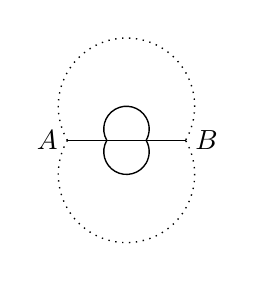
\begin{tikzpicture}[scale=0.5]
					\draw[line width=0.5pt] (0, 0) -- (3, 0);
					\node at (0, 0)[anchor = east] {$A$};
					\node at (3, 0)[anchor = west] {$B$};
					\draw[line width=0.5pt,dotted] (0,0) arc (210:-30:1.732);
					\draw[line width=0.5pt,dotted] (0,0) arc (-210:30:1.732);
					\draw[line width=0.5pt] (1,0) arc (210:-30:0.577);
					\draw[line width=0.5pt] (1,0) arc (-210:30:0.577);
				\end{tikzpicture}
			\end{figure}
		}{
			因為小編眼殘,以為題目是問垂心的軌跡,所以以下也補充了$H$的軌跡。

			我們先來證明以下事實:令$H^\prime$為$H$對$\overline{AB}$的對稱點,則$H^\prime$在$\triangle ABC$的外接圓上。
			\begin{proof}[證明]
				因為$H^\prime$為$H$對$\overline{AB}$的對稱點,所以$\angle AH^\prime B = \angle AHB = \ang{180} - \angle ACB$。於是$\angle AH^\prime B + \angle ACB=\ang{180}$,即$A, B, C, H^\prime$四點共圓。因此,$H^\prime$在$\triangle ABC$的外接圓上。
			\end{proof}
			所以,當我們知道$C$在哪裡時,只要畫出其對$\overline{AB}$的高和$\triangle ABC$外接圓的交點(就是$H^\prime$),再找出這個交點對$\overline{AB}$的對稱點就好了。因此,$H$的軌跡即為
			\begin{figure}[H]
				\centering
				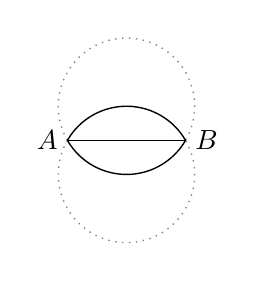
\begin{tikzpicture}[scale=0.5]
					\draw[line width=0.5pt] (0, 0) -- (3, 0);
					\node at (0, 0)[anchor = east] {$A$};
					\node at (3, 0)[anchor = west] {$B$};
					\draw[line width=0.5pt,color=gray,dotted] (0,0) arc (210:-30:1.732);
					\draw[line width=0.5pt,color=gray,dotted] (0,0) arc (-210:30:1.732);
					\draw[line width=0.5pt] (0,0) arc (-150:-30:1.732);
					\draw[line width=0.5pt] (0,0) arc (150:30:1.732);
				\end{tikzpicture}
			\end{figure}
		}
	\end{parts}
\end{questions}

\end{document}